
\chapter{局部血液循环障碍}

\chapterabstract{本章主要介绍局部血液循环障碍的类型、成因和主要病理变化。要求掌握淤血的概念和病理变化,血栓形成的概念、条件、血栓的形态特点以及血栓栓塞的后果;熟悉淤血的原因和后果,血栓的结局和对机体的影响,栓塞的概念、栓子运行的途径和脂肪栓塞的后果,梗死的概念、形成的条件、类型及病理变化;了解充血、出血的概念及病变特点,血栓形成的机制和过程。}

血液循环障碍分为全身性和局部性两种。全身性血液循环障碍发生于整个心血管系统,如休克、心力衰竭等。局部血液循环障碍发生于个别器官或局部组织,主要表现为局部血液量的异常(如充血、淤血和缺血)、血液性状和血管内容物的异常(如血栓形成、栓塞和梗死)和血管壁通透性与完整性异常(如水肿、积液和出血)。局部血液循环障碍及其所引起的病变是许多疾病过程中的基本病理改变,本章主要介绍充血、出血、血栓形成、栓塞和梗死等。
\section{充血}

局部组织和器官的血管内血液含量增多称为充血(hyperemia)。充血按其发生原因及机制不同,可分为动脉性充血和静脉性充血两类。

\subsection{动脉性充血}

局部组织和器官由于动脉血输入增多而发生的充血,称为动脉性充血(arterial
hyperemia),又称主动性充血(active hyperemia),简称充血。

\subsubsection{原因及类型}

充血可以是生理性的,也可以是病理性的。当血管舒张神经兴奋性增高或血管收缩神经兴奋性减弱时,血管就发生扩张引起充血。

\paragraph{生理性充血}
为适应器官和组织生理需要和代谢功能增强所发生的充血,称为生理性充血,如进食后的胃肠黏膜充血,体力活动时的骨骼肌充血,情绪冲动时的面颈部充血以及妊娠时的子宫充血等。

\paragraph{病理性充血}
指各种病理状态下的充血,主要有以下几种类型。

(1)炎症性充血:炎症早期,由于致炎因子刺激通过神经轴索反射使血管舒张神经兴奋,以及一些炎症介质的作用而引起的充血,称为炎性充血。

(2)减压后充血:局部器官或组织长期受压而缺血时,一旦压力突然解除,细动脉发生反射性扩张而引起充血,称为减压后充血。如绷带包扎肢体或腹水压迫腹腔内器官,组织内的血管张力降低,若迅速解开绷带或抽出大量腹水,局部受压组织的细动脉发生反射性扩张,导致局部充血。

\subsubsection{病理变化}

充血局部组织或器官的小动脉和毛细血管扩张,血量增多,体积轻度增大。如发生在体表,可见局部组织颜色鲜红。由于局部细动脉扩张,血流加快,代谢旺盛,故温度升高。功能活动增强时,发生于黏膜的充血可伴有腺体或黏膜的分泌增多。

\subsubsection{后果}

动脉性充血通常是暂时性的血管反应,原因消除后,可恢复正常,一般对机体无重要影响。炎症早期的充血,一般对机体有利,仅有少数患者,可在原有血管病变(如动脉粥样硬化、脑内小动脉瘤形成等)的基础上发生血管破裂出血。

\subsection{静脉性充血}

器官或组织静脉血液回流受阻,血液淤积于小静脉和毛细血管内引起的充血,称静脉性充血(venous
hyperemia)或被动性充血(passive hyperemia),简称淤血(congestion)。

静脉性充血可分为全身性和局部性两种,均为病理性的,具有重要的临床意义。

\subsubsection{原因}

\paragraph{静脉受压}
因压迫使静脉管腔狭窄或闭塞,血液回流障碍,导致器官或组织淤血。如肿瘤压迫局部静脉引起相应组织淤血;妊娠后期增大的子宫,压迫髂静脉,可引起下肢淤血;肠扭转、肠套叠和肠疝时,肠系膜静脉受压可致肠淤血;肝硬化时增生的肝细胞结节压迫肝内静脉分支,也是引起门静脉系统器官淤血的原因之一。

\paragraph{静脉腔阻塞}
静脉血栓形成及栓塞,可阻塞静脉血液回流,局部发生淤血。但由于静脉的分支多,只有在侧支循环不能有效建立时,静脉腔的阻塞才会发生淤血。

\paragraph{心力衰竭}
由于心收缩力减弱,不能将心腔内的血液充分搏出,导致静脉回流受阻,引起淤血。如慢性风湿性心瓣膜病变、高血压病等引起左心衰竭,可导致肺静脉回流受阻,引起肺淤血。肺源性心脏病等引起右心衰竭,使腔静脉回流受阻,导致体循环淤血。全心衰竭时,则肺循环和体循环皆出现淤血。

\subsubsection{病理变化}

\paragraph{基本病变}
肉眼观,淤血的器官体积增大,重量增加,质地变实,暗紫红色。切开器官时,可流出多量的暗红色血液。发生于体表时,由于微循环的灌注量减少,血液内氧合血红蛋白含量减少而还原血红蛋白含量增加,局部皮肤和黏膜呈紫蓝色,称发绀。由于局部血流淤滞,血管扩张,散热增加,故体表温度下降。镜下见局部细静脉和毛细血管明显扩张,充满血液。有时伴有水肿或漏出性出血。
\begin{framed}
  {案例3-1}

  {【病例摘要】}

  患者,女,41岁,因心慌、胸闷2年,咳嗽、气急30天入院。既往有风湿病史,二尖瓣狭窄。近一个月来症状加重,夜间不能平卧,起初痰中带血,现在痰呈铁锈色。体检:体温37℃、脉搏105次/分,呼吸31次/分,血压140/90
  mmHg,肝、脾未超肋缘,腹部无移动性浊音,双下肢无水肿。X线检查:双肺纹理增粗,心界扩大。

  {【问题】}

  (1)该患者肺部可能有哪些病理变化?

  (2)试分析肺部病变形成机制。
\end{framed}

\paragraph{重要器官的淤血}
(1)肺淤血:多见于慢性风湿性心脏病二尖瓣狭窄的病人。当左心室舒张时,二尖瓣不能完全开放,血液淤积于左心房内,左心房压力升高,肺静脉回流受阻,引起肺淤血。肉眼观,肺体积增大,重量增加,呈暗红色。切开时,可流出较多的淡红或暗红色泡沫状液体。镜下,肺泡壁毛细血管明显扩张,充满血液,肺泡间隔增宽。肺泡腔内可有淡红色的水肿液、少量红细胞和巨噬细胞(图\ref{fig3-1})。
\begin{figure}[!htbp]
  \centering
  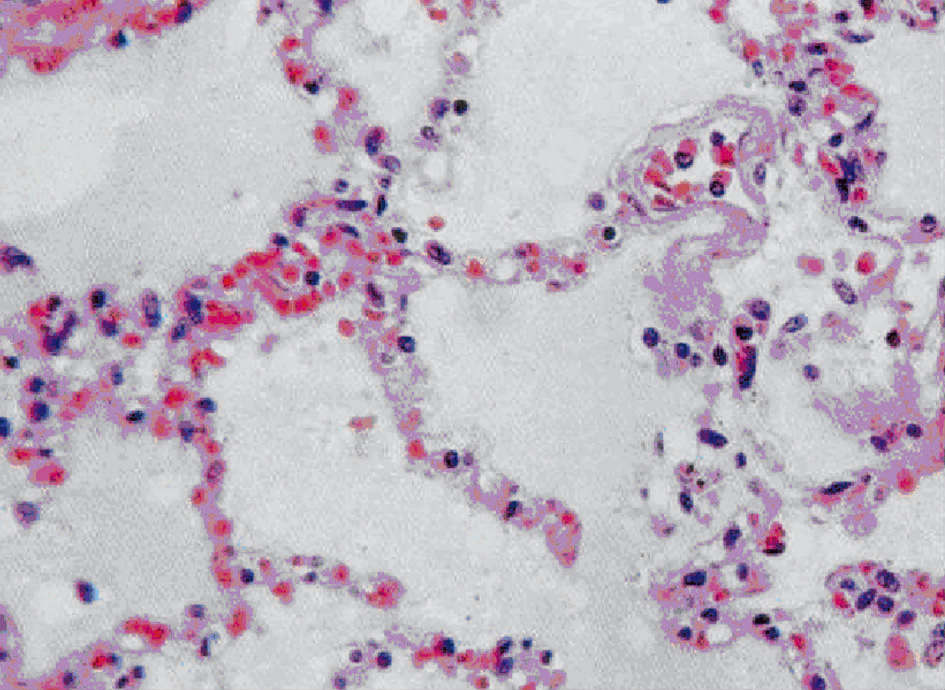
\includegraphics{./images/Image00034.jpg}
  \caption{急性肺淤血(HE染色,高倍)\\ {\small 肺泡壁毛细血管扩张充血,肺泡腔内出现大量水肿液}}
  \label{fig3-1}
\end{figure}


漏出的红细胞被巨噬细胞吞噬后,在胞浆内形成棕黄色颗粒状的含铁血黄素,这种细胞在心力衰竭时常见,故称为心衰细胞(heart
failure
cell)(图\ref{fig3-2})。长期肺淤血时,间质纤维组织增生,肺质地变硬,且伴有含铁血黄素广泛沉着,使肺组织呈现棕褐色,称之为肺褐色硬化(brown
induration)。

\begin{figure}[!htbp]
  \centering
  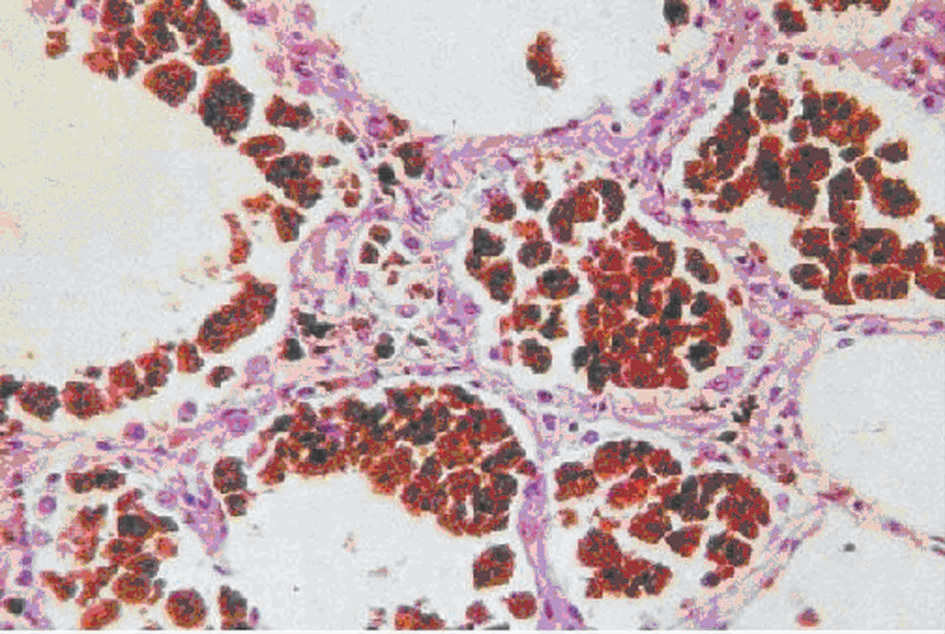
\includegraphics{./images/Image00035.jpg}
  \caption{慢性肺淤血(HE染色,高倍)\\ {\small 肺泡壁增厚纤维化,肺泡腔内见多量心衰细胞}}
  \label{fig3-2}
\end{figure}

(2)肝淤血:常由右心衰竭引起,少数也可由下腔静脉或肝静脉阻塞引起。肉眼观,肝体积增大,重量增加。切面,呈现红黄相间的花纹状结构,状似槟榔的切面,故称槟榔肝(nutmeg
liver)(图\ref{fig3-3})。镜下,肝小叶中央静脉及附近肝窦高度扩张淤血,淤血处的肝细胞受压萎缩,甚至消失。小叶周边部的肝细胞,因缺氧而发生脂肪变性。临床上,病人可因肝肿大,包膜紧张,刺激感觉神经末梢引起肝区疼痛或压痛;肝细胞损害可引起相应的肝功能障碍。长期肝淤血时,由于缺氧引起肝内纤维组织增生,最终导致淤血性肝硬化(congestive
liver cirrhosis)。

\begin{figure}[!htbp]
  \centering
  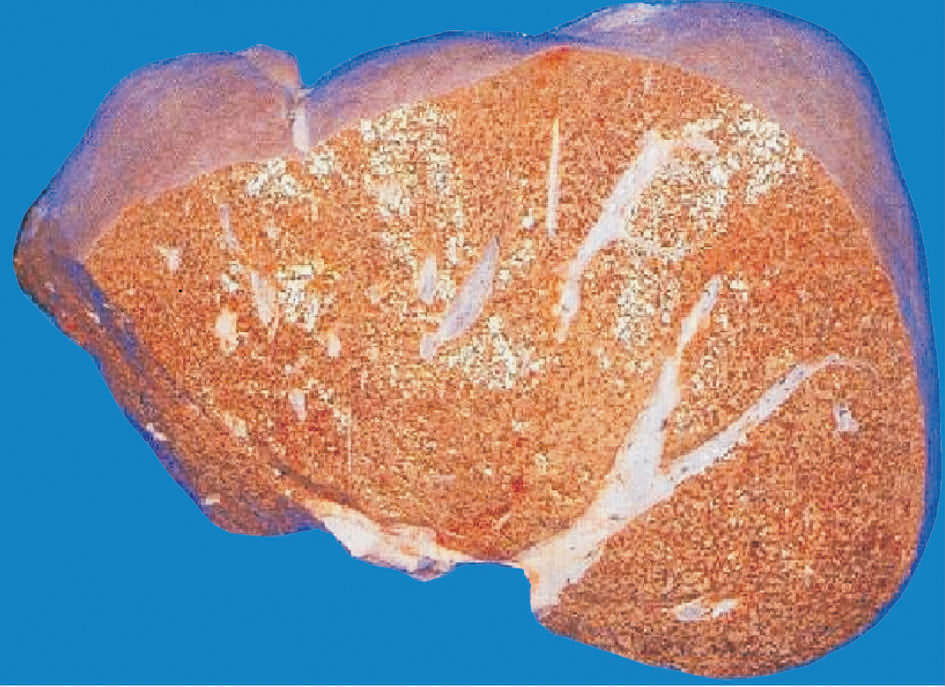
\includegraphics{./images/Image00036.jpg}
  \caption{慢性肝淤血(槟榔肝)\\ {\small 肝切面呈红黄相间的花纹状结构,似槟榔的切面}}
  \label{fig3-3}
\end{figure}

(3)脾淤血:常见于肝硬化或心力衰竭时,亦可在脾静脉和门静脉血栓形成时发生。肉眼观,脾脏体积增大,重量增加。切面呈暗红色,脾小体明显可见。近包膜处可见散在针头大小黄褐色结节,称之为含铁结节(siderotic
nodules)。镜下,脾窦扩张淤血,窦壁增厚,脾索纤维化及增粗。脾髓内巨噬细胞增多,胞浆内多有含铁血黄素。含铁结节由游离的含铁血黄素与钙盐、铁盐结合在结缔组织中灶性沉积形成。

\subsubsection{后果}

淤血的后果取决于静脉阻塞发生的速度、程度、部位、淤血持续的时间以及侧支循环建立的情况等因素。

\paragraph{淤血性水肿和出血}
淤血持续时间较长时,由于血流缓慢及缺氧,使毛细血管壁通透性升高,毛细血管内流体静压升高,血液的液体成分漏出增多,形成淤血性水肿。这种水肿液的蛋白质含量低,细胞数少,称为漏出液。严重时,红细胞亦可漏出,引起点状或斑状出血。

\paragraph{实质细胞萎缩、变性和坏死}
长期淤血的组织由于缺氧,组织中氧化不全产物堆积,可引起实质细胞的萎缩、变性,甚至坏死。

\paragraph{淤血性硬化}
由于长期淤血,间质内纤维组织增生,组织内原有的网状纤维融合变成胶原纤维,使器官变硬,称为无细胞性硬化。常见于肺、肝及脾的慢性淤血。

\paragraph{侧支循环开放}
肝硬化时,由于门静脉慢性淤血,部分血液可经过开放的静脉吻合支回流至上、下腔静脉,导致食管下段静脉曲张、脐周腹壁静脉曲张和痔静脉丛曲张。侧支循环开放虽然有代偿静脉回流的作用,但因侧支静脉过度曲张,有时可发生破裂,甚至引起大出血。

\section{出血}

血液从心腔或血管逸出,称为出血(hemorrhage)。逸出的血液进入组织间隙或体腔,称为内出血。血液流出到体外,称为外出血。

\subsection{原因和发病机制}

按血液逸出的机制可分为破裂性出血和漏出性出血。

\subsubsection{破裂性出血}

心脏或血管破裂引起的出血,称破裂性出血。多见于外伤或心脏、血管壁病变。如动脉粥样硬化、心肌梗死的室壁瘤等。此外,如结核病变对血管壁的损伤,恶性肿瘤侵犯血管壁等,均可引起破裂性出血。

\subsubsection{漏出性出血}

毛细血管与细静脉的通透性升高,血液通过增大的内皮细胞间隙及损伤的基底膜缓慢地漏出血管外,称漏出性出血。临床上称之为“渗血”。其相关因素有:

\paragraph{血管壁的损害}
常由于淤血、缺氧、感染、中毒等因素的损害引起。如淤血和缺氧时,毛细血管内皮细胞因缺氧发生变性,酸性代谢产物损伤基底膜和毛细血管内流体静压升高等可引起出血;败血症、流行性出血热、钩端螺旋体病、蛇毒及有机磷中毒等均可致毛细血管壁损伤,通透性增强,引起出血;维生素C缺乏时毛细血管内皮细胞接合处的基质和血管外的胶原基质形成降低,使血管脆性和通透性增加而引起出血;某些药物或食物可使机体产生过敏反应而损伤毛细血管,使血管壁通透性增高引起出血等。

\paragraph{血小板减少或功能障碍}
如血小板减少性紫癜、血小板功能缺陷、脾功能亢进、再生障碍性贫血、急性白血病等,均可致漏出性出血。

\paragraph{凝血因子缺乏}
如凝血因子Ⅷ(血友病A)、Ⅸ(血友病B)、von
Willebrand因子缺乏、纤维蛋白原、凝血酶原等因子的先天性缺乏;维生素K缺乏、严重肝脏疾病等,引起凝血因子合成减少;弥散性血管内凝血(DIC)时,凝血因子消耗过多等,均可引起继发性广泛出血。

\subsection{病理变化}

内出血可见于体内任何部位,发生在体腔称积血,如胸腔积血、腹腔积血、心包积血、蛛网膜下腔出血等(图\ref{fig3-4})。体腔内可见血液与凝血块。出血发生在组织间隙时,可见多少不等的红细胞散在其中,如多量血液聚集形成局限性肿块,则称为血肿,如脑硬膜下血肿、皮下血肿、脑实质血肿等。皮肤、黏膜、浆膜等处有微小出血时,在局部形成淤点或淤斑。

外出血时,在伤口处可见血液外流或形成血凝块。鼻黏膜出血排出体外称鼻衄;支气管或肺出血经口排出到体外称为咯血;食管或胃出血经口排出到体外称为呕血;结肠、胃出血经肛门排出称便血;泌尿道出血经尿道排出称尿血。

\subsection{后果}

出血的后果主要取决于出血类型、出血量、出血速度和出血部位。人体具有止血的功能,缓慢而少量的出血,多可自行止血。局部组织或体腔内的血液,可通过吸收、机化或纤维包裹而阻止继续出血。一般少量内出血可被巨噬细胞清除不留痕迹;如出血量较多,则多量血色素被巨噬细胞吞噬,分解为含铁血黄素或橙色血质,长期留存组织内,缓慢吸收、转运。少量漏出性出血一般不引起严重后果,但如范围广泛,亦可造成严重影响。破裂性出血如发生在较大血管,短时间内出血量达到总血量的20%~25%,可致出血性休克;如发生在重要器官如脑,常可造成严重后果;少量慢性反复出血可引起缺血性贫血。

\begin{figure}[!htbp]
  \centering
  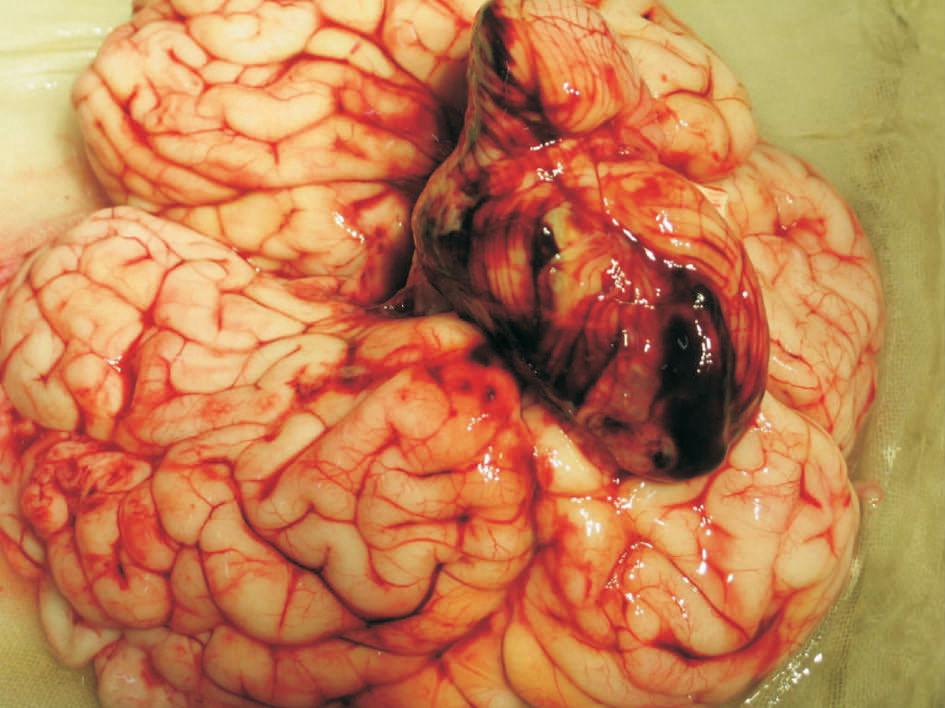
\includegraphics{./images/Image00037.jpg}
  \caption{小脑蛛网膜下腔出血}
  \label{fig3-4}
\end{figure}


\section{血栓形成}

在活体的心脏和血管内,血液发生凝固或血液中某些有形成分析出凝集形成固体质块的过程,称为血栓形成(thrombosis),所形成的固体质块称为血栓(thrombus)。

血液中存在着相互拮抗的凝血系统和纤维蛋白溶解系统。在生理状态下,血液中的凝血因子不断被激活,从而产生凝血酶,形成微量纤维蛋白,沉着于血管内膜。这些纤维蛋白又不断地被激活了的纤维蛋白溶解系统所溶解。同时被激活的凝血因子也不断地被单核巨噬细胞系统所吞噬。这种凝血系统与纤维蛋白溶解系统的动态平衡,既保证了血液有潜在的可凝固性,又始终保证了血液的流体状态。上述动态平衡一旦被打破,触发了凝血过程,血液便可以在心血管腔内凝固,进而形成血栓。

\subsection{血栓形成的条件和机制}

血栓形成是血液在心血管内流动情况下所发生的血液凝固。它是在一定条件下通过血小板的析出、黏集和血液凝固几个基本过程形成的。其形成条件主要有以下三个方面:

\subsubsection{心血管内膜损伤}

心血管内膜的内皮细胞具有抗凝和促凝的两种特性,在正常情况下,以抗凝作用为主,从而使心血管内血液保持流体状态。心血管内膜损伤是血栓形成最重要和最常见的条件。内皮细胞损伤后,暴露出内皮下胶原,激活血小板和凝血因子Ⅻ,启动内源性凝血系统。同时,损伤的内皮细胞释放组织因子,激活血小板因子Ⅶ,启动外源性凝血系统。

血小板活化在促发凝血和血栓形成过程中的作用极其重要,主要表现为以下三项反应:

\paragraph{黏附反应(adhesion)}
血小板经过变形,由细胞骨架微丝和微管形成伪足,黏附于暴露出的内皮下胶原。毛细血管基底膜、纤维母细胞和平滑肌细胞均有黏附血小板的作用,但以胶原的黏附作用最强。

\paragraph{释放反应(release reaction)}
黏附后的血小板可以释放ADP、5-HT、血小板生长因子、血栓素A2(thromboxane
A2,TXA2)等促凝物质。其中ADP和TXA2与血栓形成关系最为密切。

\paragraph{黏集反应(aggregation)}
血小板除了与内皮下胶原黏附外,还可与纤维蛋白和纤维连接蛋白黏附,促使血小板彼此黏集成堆,称为血小板黏集堆。最初血小板黏集是可逆的,随着内源性和外源性凝血系统的激活、凝血酶的形成,使血小板黏集堆变成不可逆性,成为血栓形成的起始点。

心血管内膜损伤的原因主要有细菌、病毒感染、内毒素、酸中毒、免疫复合物和理化因素等。其引起血栓形成,多见于风湿性或感染性心内膜炎病变的心瓣膜上、动脉硬化之粥瘤性溃疡、心肌梗死区域的心内膜、动脉或静脉内膜炎及创伤性血管损伤部位等。

\subsubsection{血流状态的改变}

血流状态的改变主要指血流缓慢及产生涡流等改变,有利于血栓形成。正常情况下,血流速度较快,血液中的有形成分如红细胞、白细胞及血小板,均在血流的中轴部流动,构成轴流,其外周为血浆,构成边流。当血流缓慢或产生涡流时,则轴流消失,使血小板易与受损的血管内膜接触而发生黏集。而且血流缓慢时,被激活的凝血因子和凝血酶易在局部积聚而浓度增高,激发凝血过程。因此,血栓多发生于血流较缓慢的静脉内。据统计,发生于静脉内的血栓,约比动脉内的多4倍;下肢静脉内的血流受重力的影响较上肢大,血栓形成的机会比上肢静脉多3倍。静脉血栓常发生于心力衰竭、久病卧床的病人,因全身血流缓慢等因素,易致血栓形成。心脏和动脉的血流快,不易形成血栓,但在血流较缓和出现涡流时,也会有血栓形成。如二尖瓣狭窄时的左心房、动脉瘤内管腔膨出产生涡流,有利于血小板析出和黏集,容易形成血栓。

\subsubsection{血液凝固性增加}

血液凝固性增加主要是指血液中血小板和凝血因子增多,或纤维蛋白溶解系统活性降低,导致血液的高凝状态。可见于一些遗传性和获得性疾病。在遗传性高凝状态的原因中,第Ⅴ因子和凝血酶原的基因突变最为常见。有报道在复发性深静脉血栓形成的病人中,第Ⅴ因子基因突变出现率高达60%。患有原发性高凝状态的病人,也可能与遗传性凝血酶Ⅲ、蛋白C或蛋白S的缺乏有关。在获得性高凝状态疾病中,如胃肠道、胰腺、肺和卵巢等器官的黏液癌发生广泛转移时,由于癌细胞释放出促凝因子入血,引起弥散性血管内凝血(DIC)。在大面积烧伤、严重创伤、产后或大手术后,由于严重失血,血液浓缩,血液中纤维蛋白原、凝血酶原、凝血因子Ⅻ、凝血因子Ⅶ等含量增多,以及血中补充大量幼稚的血小板,具有较高的黏性,易发生黏集形成血栓。血小板增多或黏性增高还可见于妊娠中毒症、高脂血症、冠状动脉粥样硬化以及吸烟和肥胖症等。

血栓形成往往是多种因素综合作用的结果(图\ref{fig3-5})。上述三种条件,常常同时存在,相互影响,协同作用,或是其中某一条件起主要作用。如心力衰竭病人,除血流缓慢外,还可因缺氧使血管内皮细胞发生损伤,受损伤的血管内皮细胞又可释放组织凝血因子,使血液凝固性增高。再如,某些外伤或手术后病人,除血管内膜损伤外,还伴有血流状态改变及血液性质变化,易致血栓形成。

\begin{figure}[!htbp]
  \centering
  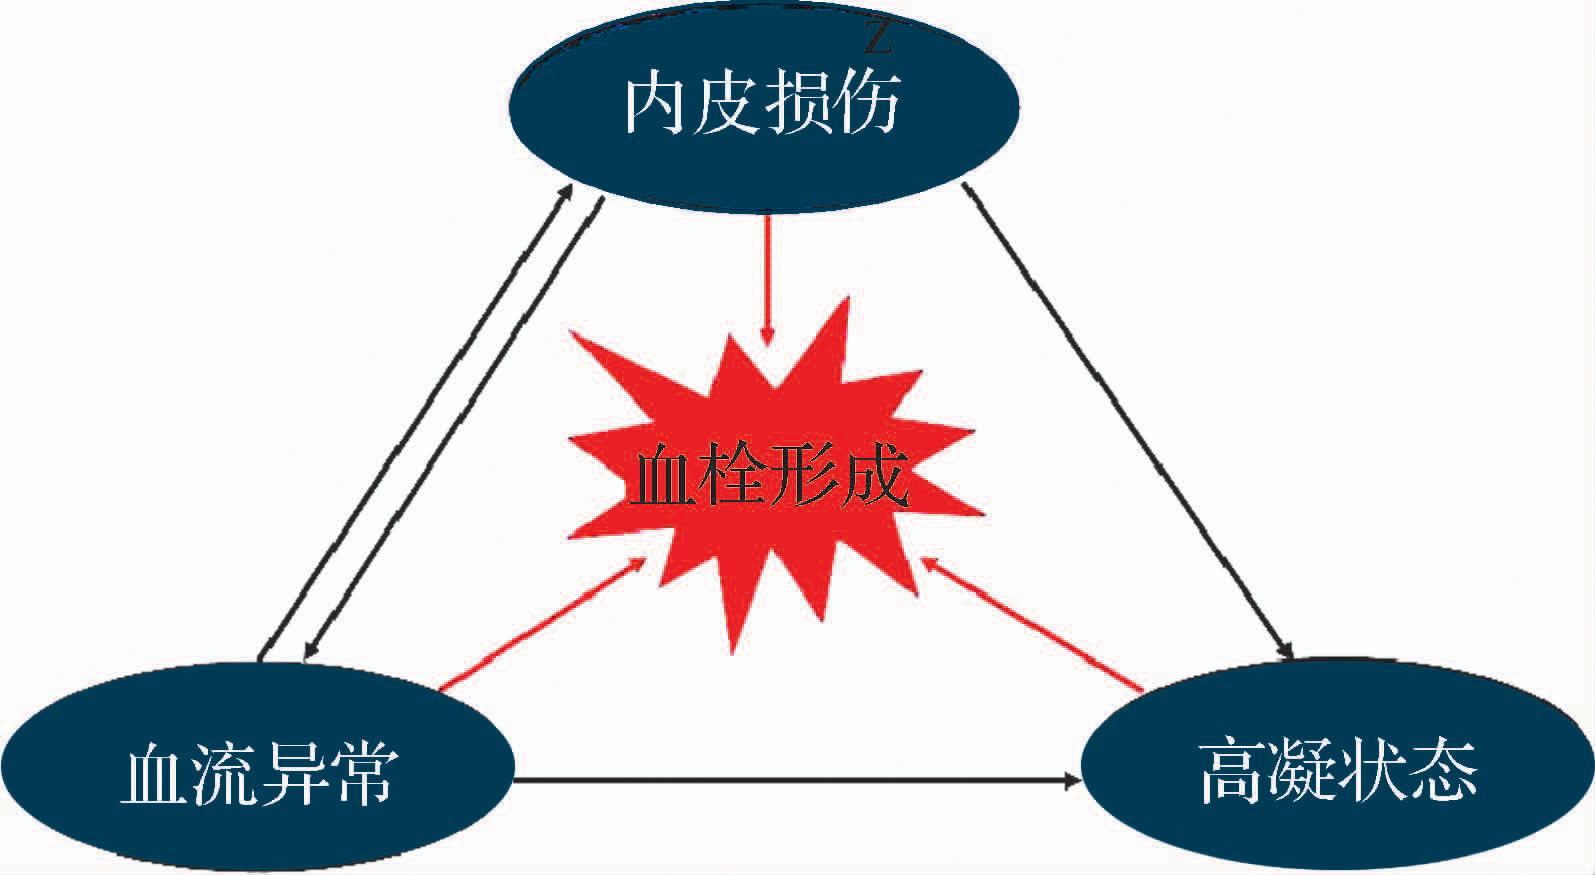
\includegraphics{./images/Image00038.jpg}
  \caption{多因素综合作用导致血栓形成}
  \label{fig3-5}
\end{figure}

\subsection{血栓形成的过程及血栓的形态}

血栓形成的过程主要包括血小板黏附、凝集和血液成分凝固几个阶段(图\ref{fig3-6})。无论心脏或血管的血栓,其形成过程都是以血小板黏附于内膜裸露的胶原开始。因此,血小板黏集堆的形成是血栓形成的第一步,嗣后血栓形成的过程及血栓的组成、形态、大小都取决于血栓发生的部位和局部血流速度。血栓的类型可分为以下四种:

\begin{figure}[!htbp]
  \centering
  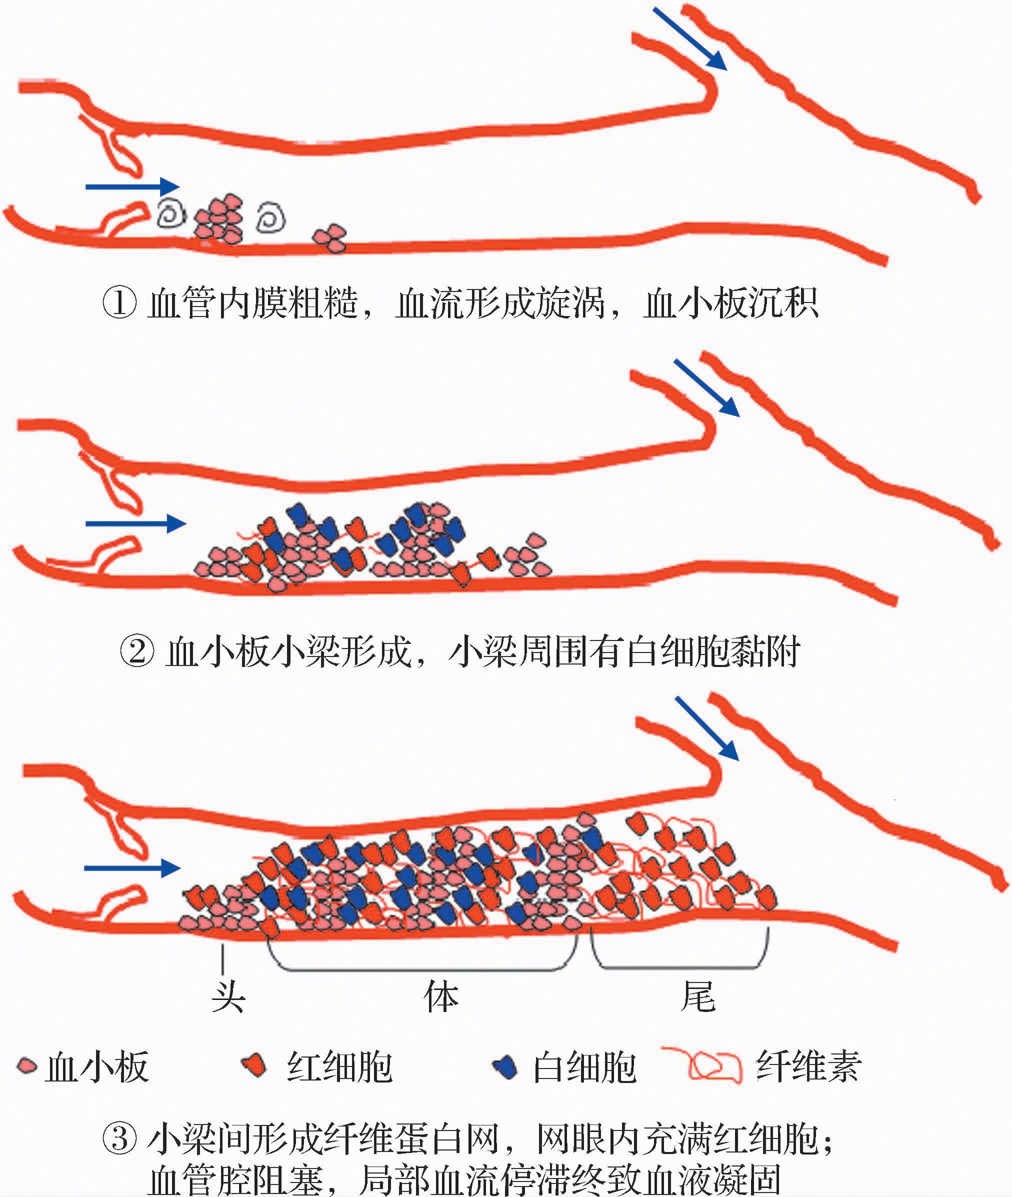
\includegraphics{./images/Image00039.jpg}
  \caption{静脉内血栓形成过程示意图}
  \label{fig3-6}
\end{figure}

\subsubsection{白色血栓}

白色血栓(pale
thrombus)是由血小板黏附、黏集形成的附着于心血管壁损伤处的血栓。多发生于血流较快的心瓣膜、心腔内、动脉内或静脉性血栓的起始部,即延续性血栓的头部。肉眼观,呈灰白色小结节或赘生物状,表面粗糙、质较坚实,与心血管壁紧密黏着,不易脱落。镜下,主要由血小板及少量纤维素构成,又称血小板血栓或析出性血栓。

\subsubsection{混合血栓}

静脉血栓在形成血栓头部后,其下游的血流进一步减缓并形成涡流,在血管腔内形成新的血小板小梁的黏集堆。在血小板小梁之间的血液发生凝固,纤维蛋白形成网状结构,网内充满大量的红细胞。这一过程反复交替进行,致使形成的血栓在肉眼观时呈灰白色和红褐色层状交替结构,称为层状血栓,即混合血栓(mixed
thrombus)。构成静脉内延续性血栓的体部。肉眼观,混合血栓呈粗糙干燥圆柱状,与血管壁粘连,有时可辨认出不规则的灰白和褐色相间的条纹状结构。发生于心腔内、动脉粥样硬化溃疡部位或动脉瘤内的混合血栓,可称为附壁血栓。镜下,混合血栓主要由淡红色无结构的不规则分枝状或珊瑚状的血小板小梁和小梁间充满红细胞的纤维素网所构成,并见血小板小梁边缘有较多中性粒细胞黏附(图\ref{fig3-7})。

\begin{figure}[!htbp]
  \centering
  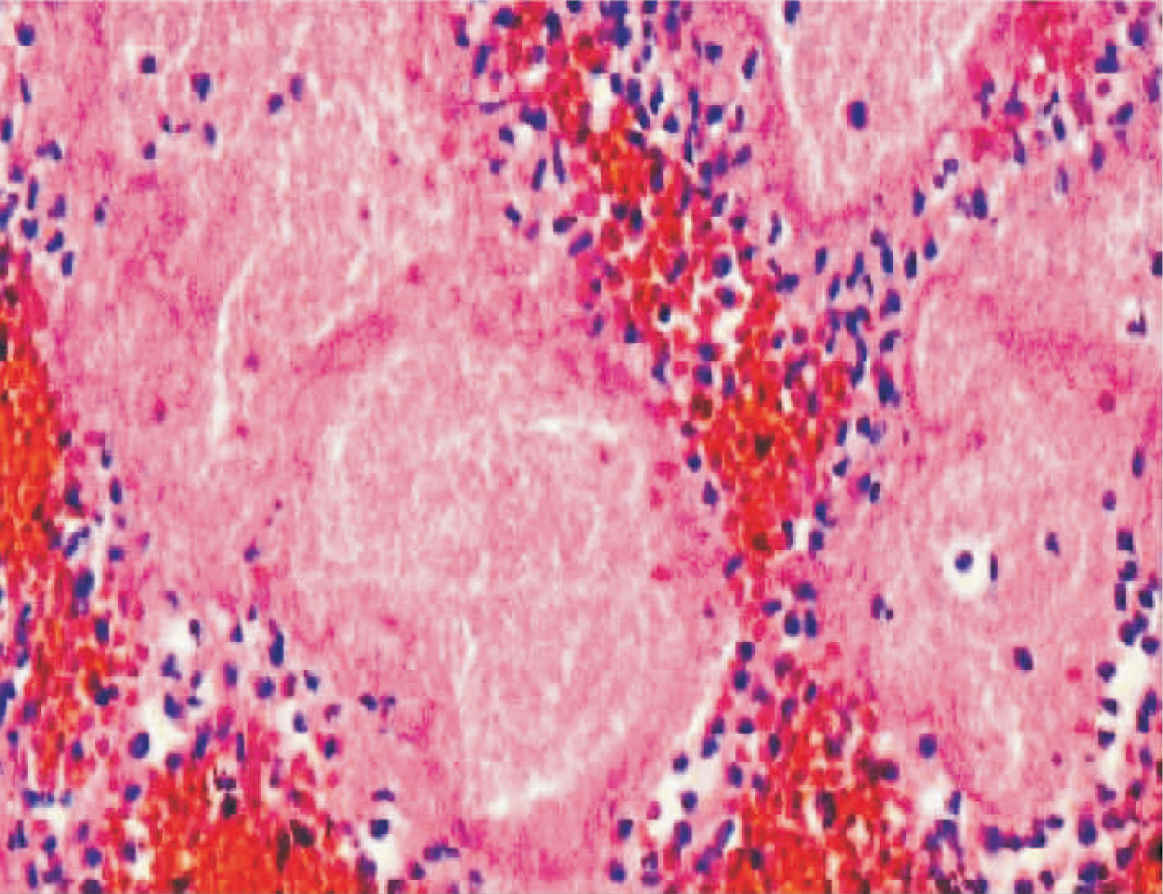
\includegraphics{./images/Image00040.jpg}
  \captionsetup{justification=centering}
  \caption{混合血栓镜下结构(HE染色,高倍) \\ {\small 珊瑚状血小板小梁边缘有白细胞黏附,小梁之间为纤维蛋白网和红细胞}}
  \label{fig3-7}
\end{figure}

\subsubsection{红色血栓}

红色血栓(red
thrombus)主要见于静脉,随着静脉血栓逐渐增大并阻塞管腔,使血流下游局部血流停止,血液迅速发生凝固,形成红色血栓,常构成延续性血栓的尾部。红色血栓的形成过程与血管外凝血过程相同。肉眼观,呈暗红色、湿润、有弹性、与血管壁无粘连,与死后血凝块相似。陈旧的红色血栓由于水分被吸收而变得干燥、无弹性、质脆易碎,可脱落造成栓塞。镜下,在纤维素网眼内充满如正常血液分布的血细胞。

\subsubsection{透明血栓}

透明血栓(hyaline
thrombus)发生于微循环的血管内,主要在毛细血管,因其只能在显微镜下见到,故又称微血栓。透明血栓主要由嗜酸性同质性的纤维蛋白构成,又称为纤维素性血栓。这种血栓为多发性,最常见于弥散性血管内凝血(DIC)时的微循环内。微血栓形成后,还会继发性激活纤维蛋白溶解系统,使微血栓溶解,故后期在病理切片中有时又难以见到微血栓。

各种类型血栓的常见部位及其形态特点见表\ref{tab3-1}。

\begin{table}[ht]
  \caption{各种血栓的常见部位及形态特点}
  \label{tab3-1}
  \centering
  \begin{tabular}{lp{4cm}p{4cm}p{4cm}}
    \toprule
    血栓类型                                    & 常见部位                                                                      & 肉眼特点                                                    & 镜下特点 \\
    \midrule
    白色血栓                                    & 心瓣膜、动脉内、延续性血栓头部                                                &
    灰白色,表面粗糙 、质坚实,与心血管壁紧密粘着 & 主要 成分为血小板及少量纤维蛋白                                                                                                                        \\
    混合血栓                                    & 心腔内、 动脉内、延续性血栓体部
                                                & 质较实, 干燥,呈红白相间条纹状,与血管壁黏连较紧密                             & 血小板小梁 上附有中性粒细胞与纤维蛋白网罗大量红细胞交错排列            \\
    红色血栓                                    & 静脉内、延续性血栓尾部
                                                & 新鲜时,暗红、湿润、有弹性与,血管壁无粘连;陈旧时,暗红、干燥、无弹性、质脆易碎
                                                & 纤维素网眼内充满如正常血液分布的血细胞                                                                                                                 \\
    透明血栓                                    & 微循环小血管内                                                                & 肉眼观察不到                                                &
    主要由纤维蛋白构成,有少量血小板,呈均质红染状态                                                                                                                                                      \\
    \bottomrule
  \end{tabular}
\end{table}

\subsection{血栓的结局}

\subsubsection{软化、溶解与吸收}

血栓形成后,由于纤维蛋白溶解系统的作用,以及血栓内白细胞崩解后释放溶蛋白酶,使血栓发生软化、溶解,变成细小颗粒或液体。它可被血流冲走,或被吞噬细胞吞噬。较小的血栓,可被完全溶解吸收而不留痕迹。较大的血栓多发生部分软化和溶解,在血流的冲击作用下,整个血栓或血栓的一部分,可脱落成为血栓性栓子,随血流运行至组织器官中,引起该部位血管腔的阻塞,造成血栓栓塞。

\subsubsection{机化与再通}

在血栓形成后的1~2天,已开始有内皮细胞、纤维母细胞和肌纤维母细胞从血管壁长入血栓并逐渐取代血栓。这种由肉芽组织逐渐取代血栓的过程,称为血栓机化。中等大小的血栓经两周左右即可完成机化,此时血栓与血管壁紧密粘连不再脱落。在血栓机化的同时,由于水分被吸收,血栓干燥而出现裂隙,血管内皮细胞可以生长覆盖于裂隙的表面而形成新的血管,管腔之间可以相互吻合沟通,使被阻断的血流部分地恢复重建。这一过程称为再通(recanalization)(图\ref{fig3-8})。

\begin{figure}[!htbp]
  \centering
  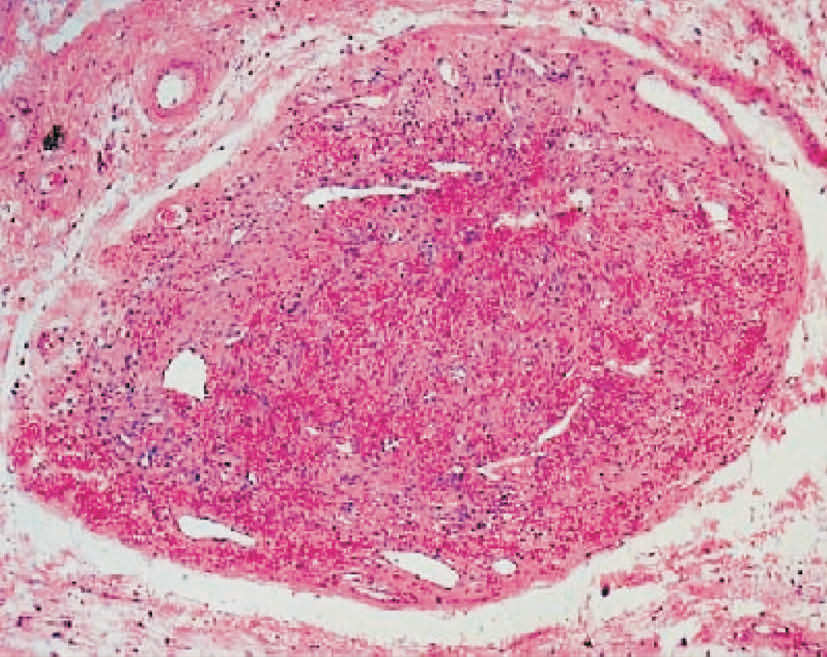
\includegraphics{./images/Image00042.jpg}
  \caption{血栓机化与再通(HE染色,低倍) \\ {\small 血管内血栓被肉芽组织取代,并再通}}
  \label{fig3-8}
\end{figure}


\subsubsection{钙化}

如血栓未发生软化或机化,则钙盐可在血栓内沉积,使血栓部分或全部钙化成坚硬的质块。此种情况如发生在静脉内,称为静脉石。

\subsection{血栓对机体的影响}

血栓形成对破裂的血管起阻塞裂口和止血作用,这是对机体有利的一面。在某些病理情况下,如肺结核空洞壁和慢性消化性溃疡底部的血管,在病变侵蚀前常已形成血栓,避免了因这些血管损伤而造成大出血的可能性。又如,炎症灶小血管内有血栓形成,可以防止病原体经血管蔓延扩散。因此,在一定条件下,血栓形成可看做是机体的一种防御性措施。但多数情况下血栓形成对机体则造成不利的影响。

\subsubsection{阻塞血管}

血栓形成对机体的危害主要是阻塞血管,引起血液循环障碍。其影响的大小,取决于血栓发生的部位、阻塞血管供血的范围、阻塞的程度以及能否有效地建立侧支循环等因素。当动脉管腔因闭塞性血栓而完全被阻塞,同时又缺乏有效的侧支循环代偿时,则局部组织可因缺血而坏死(梗死)。如脑动脉血栓引起脑梗死,心冠状动脉血栓引起心肌梗死,以及股动脉闭塞性脉管炎引起足趾坏疽等。静脉血栓形成,若未能建立有效的侧支循环,则因静脉回流障碍引起局部组织器官淤血、水肿、出血,甚至坏死。如肠系膜静脉血栓可引起肠的出血性梗死等。

\subsubsection{栓塞}

血栓的整体或部分脱落形成栓子,随血流运行可引起栓塞。若栓子内含有细菌,可引起败血性梗死或脓肿形成。

\subsubsection{心瓣膜病}

血栓引起的心瓣膜病见于心内膜炎。心瓣膜上反复发作的血栓形成及机化,可使瓣膜瓣叶粘连增厚变硬,腱索增粗缩短,引起瓣口狭窄或关闭不全,导致慢性心瓣膜病。严重时,可致心力衰竭并导致全身血液循环障碍。

\subsubsection{出血}

血栓引起的出血见于DIC时,微循环内广泛性透明血栓形成,可引起全身广泛性出血和休克。

\section{栓塞}

在循环血液中出现不溶于血液的异常物质,随血流运行阻塞血管腔的现象,称为栓塞(embolism)。阻塞血管腔的异常物质称为栓子(embolus)。栓子可为固体、液体或气体。最常见的是血栓栓子,其他还有脂肪滴、气体、羊水、细菌以及肿瘤细胞栓子等。

\subsection{栓子运行的途径}

栓子一般随血流方向运行(图\ref{fig3-9})。

\begin{figure}[!htbp]
  \centering
  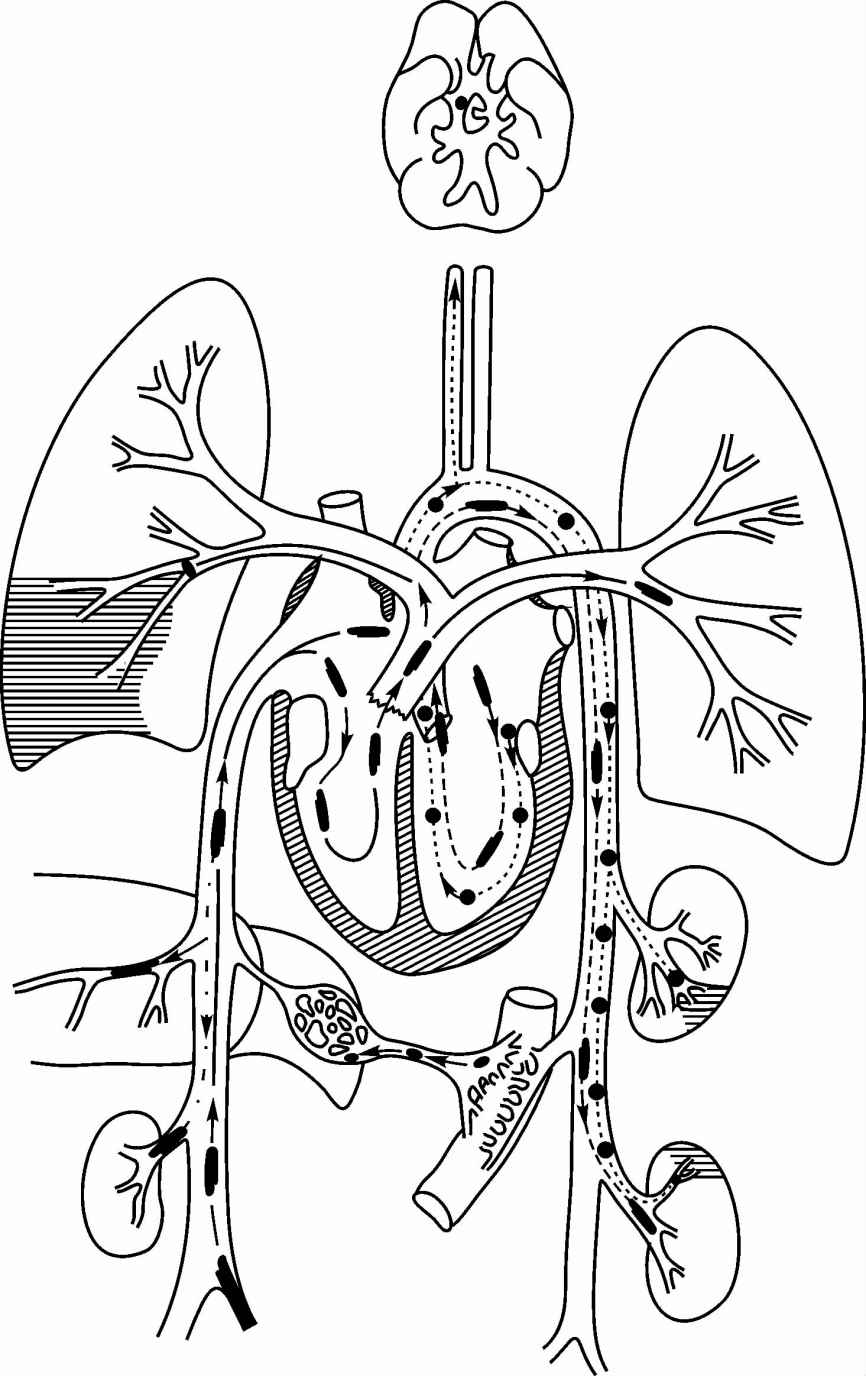
\includegraphics{./images/Image00043.jpg}
  \caption{栓子运行途径与栓塞模式图}
  \label{fig3-9}
\end{figure}

\paragraph{来自体静脉系统及右心的栓子}
随血流进入肺动脉主干及其分支,可引起肺栓塞。某些体积小的脂肪、气体或羊水栓子,因为具有一定的弹性,可通过肺循环进入体循环系统,继而引起动脉分支的栓塞。

\paragraph{来自左心或主动脉系统的栓子}
随动脉血流运行,阻塞于各器官的小动脉内引起栓塞。常见于脑、脾、肾等器官。

\paragraph{来自肠系膜静脉等门静脉系统的栓子}
常在肝内门静脉的分支形成栓塞。

\paragraph{交叉性栓塞}
在先天性房、室间隔缺损或动、静脉瘘的患者,栓子可通过缺损处,由压力高的一侧进入压力低的一侧,产生动、静脉系统栓子的交叉运行,形成交叉性栓塞。

\paragraph{逆行性栓塞}
极罕见于下腔静脉内的栓子,在胸、腹腔压力急剧升高(如咳嗽等)时,可逆血流方向运行,在肝静脉、肾静脉等分支内形成逆行性栓塞。

\subsection{栓塞的类型和对机体的影响}

栓塞有以下几种类型,其对机体的影响,取决于栓子的类型与大小、栓塞的部位以及侧支循环建立的状况等。

\subsubsection{血栓栓塞}

由血栓或血栓的一部分脱落造成的栓塞,称为血栓栓塞(thromboembolism)。血栓栓塞是栓塞最常见的原因,占全部栓塞的99%以上。由于血栓栓子的来源、大小和栓塞部位的不同,对机体的影响也有所不同。

\begin{framed}
  {案例3-2}

  {【病例摘要】}

  患者,男性,67岁,因前列腺癌住院手术治疗。术后第6天下床活动,步行去洗手间回来,刚刚走到病床边,便突然晕倒,继而呼吸、心跳停止,经抢救无效死亡。

  {【尸检摘要】}

  在肺动脉分叉处见一枚长约15
  cm的条状固体质块骑跨于左右肺动脉口,两端暗红色,中间部分可见多数灰白色条纹。镜下观:肺动脉腔内的固体质块主要为崩解的血小板构成的小梁,小梁间为纤维蛋白网和红细胞,小梁边缘见较多白细胞附着。

  {【问题】}

  (1)本例的病理诊断是什么?

  (2)阻塞肺动脉的固体质块最可能来源于何处?

  (3)造成病人死亡的可能机制是什么?
\end{framed}

\paragraph{肺动脉栓塞}
造成肺动脉栓塞的血栓栓子95%以上来自下肢深部静脉,尤其是腘静脉、股静脉和髂静脉,偶可来自盆腔静脉或右心附壁血栓。根据栓子的大小和数量,其引起栓塞的后果不同:①中小栓子仅阻塞肺动脉的少数小分支,一般不产生严重后果。因为肺具有双重血循环,特别是支气管动脉和肺动脉之间有丰富的吻合支,肺动脉可从支气管动脉得到血液供应。但在肺严重淤血时,支气管动脉侧支循环不能充分发挥作用,则可引起肺出血性梗死。②大的血栓栓子栓塞于肺动脉主干或大分支,较长的栓子可栓塞左右肺动脉干,形成骑跨性栓塞,可引起病人突然出现呼吸困难、发绀、休克等症状。严重者可因呼吸循环衰竭死亡(猝死),称为肺动脉栓塞症或肺卒中。③若栓子小但数目多,可广泛栓塞于肺动脉多数小分支,也可引起右心衰竭、猝死。

\begin{center}
  \textbf{知识链接}
\end{center}
\chapterabstract{
肺动脉栓塞引起猝死的原因尚未完全阐明。一般认为,较大栓子栓塞肺动脉主干或大分支时,肺动脉阻力急剧增加,造成急性右心衰竭;同时肺缺血缺氧,左心回心血量减少,冠状动脉灌流不足导致心肌缺血;血栓栓子刺激肺动脉管壁引起迷走神经反射,导致肺动脉、支气管动脉、冠状动脉广泛性痉挛和支气管平滑肌痉挛,进而导致急性右心衰竭和窒息;血栓栓子中的血小板释放出大量5-HT及TXA2亦可引起肺动脉的痉挛,故新鲜的血栓栓子比陈旧性血栓栓子危害性更大。
}
\paragraph{体循环动脉栓塞}
栓子80%来自左心及动脉系统的附壁血栓,如感染性心内膜炎时瓣膜上的赘生物、心肌梗死区心内膜上的附壁血栓,其余来自动脉粥样硬化粥瘤性溃疡或动脉瘤内的附壁血栓,极少数来自腔静脉的栓子,通过房室间隔缺损进入左心,引起交叉性栓塞。动脉栓塞的主要部位为下肢和脑,亦可累及肠、肾和脾。动脉栓塞的后果取决于栓子的大小、栓塞的部位和局部侧支循环情况以及组织对缺氧的耐受性。栓塞动脉分支小,又能建立有效的侧支循环,可无严重后果;若栓塞的动脉分支大,又不能建立有效的侧支循环,局部组织可发生梗死。若栓塞发生于冠状动脉或脑动脉分支,常可造成严重后果,甚至危及生命。

\subsubsection{脂肪栓塞}

在循环血流中出现脂肪滴阻塞于小血管,称脂肪栓塞(fat
embolism)。栓子来源常见于长骨骨折、脂肪组织严重挫伤和烧伤时,骨髓或脂肪组织的脂肪细胞受损破裂,脂肪游离成无数脂肪滴,通过破裂的小静脉进入血流。脂肪滴也可出现在非创伤性患者血流中,如脂肪肝、酗酒、血脂过高、急性胰腺炎患者,或在一次进食大量脂肪餐后,血中可出现游离脂肪滴,引起脂肪栓塞。

脂肪栓塞常见于肺、脑等器官,其后果取决于脂肪滴的大小及数量。直径大于20
μm的脂肪滴,可引起肺动脉分支、肺小动脉(图\ref{fig3-10})或毛细血管的栓塞。若大量脂滴短期内进入肺循环,可出现突发性的呼吸急促、心动过速,患者可因窒息或急性右心衰竭而死亡。直径小于20
μm的脂肪滴可通过肺泡壁毛细血管经肺静脉到左心进入体循环的分支,还可通过心脏未闭合的卵圆孔或动脉导管及室间隔缺损,进入体循环动脉,引起脑、肾、皮肤等全身多器官栓塞,最常见为脑血管的栓塞,引起脑水肿和血管周围点状出血,甚至发生脑梗死,患者可出现烦躁不安、谵妄和昏迷等。

\begin{figure}[!htbp]
  \centering
  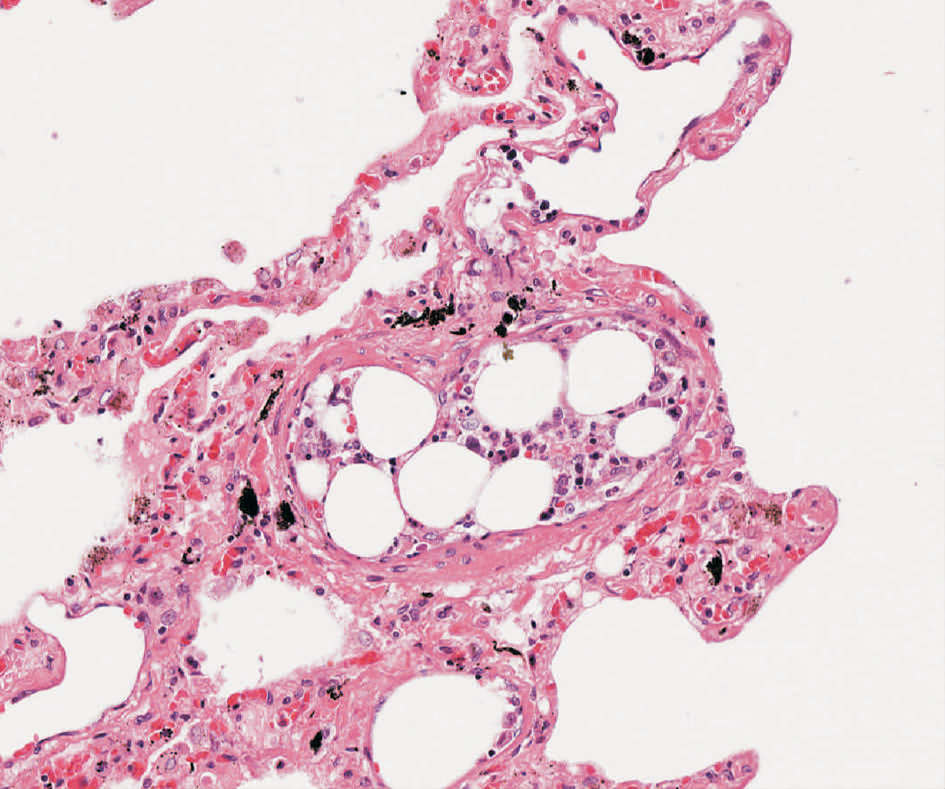
\includegraphics{./images/Image00044.jpg}
  \caption{骨折后肺小动脉分支脂肪栓塞(HE染色,中倍) \\ {\small 血管腔内见脂滴空泡和骨髓造血细胞}}
  \label{fig3-10}
\end{figure}


\subsubsection{气体栓塞}

大量气体迅速进入血循环或原溶于血中的气体迅速游离,形成气泡阻塞于心血管腔所引起的栓塞,称为气体栓塞(gas
embolism)。前者为空气栓塞(air embolism),后者称减压病。

空气栓塞多因静脉损伤破裂,外界空气通过破裂口进入血流所致。如头颈手术、胸壁和肺创伤损伤静脉、使用静脉输液、人工气胸或气腹误伤静脉时,空气可在吸气时因静脉腔内的负压吸引,由损伤口进入静脉。亦可见于分娩或流产时,子宫强烈收缩,将空气挤入子宫壁破裂的静脉窦内。

空气进入血循环的后果取决于进入的速度和气体量。少量空气进入血流,可很快被吸收或溶解于血液内,不引起栓塞。若大量气体(>100
ml)迅速进入静脉,随血流到右心后,因心脏搏动和血流冲击将空气与血液搅拌形成大量气泡,这种泡沫状血液有很高的弹性,可随心脏的收缩、舒张而压缩或膨胀,从而阻止了静脉血的回流和向肺动脉的输出,造成严重的循环障碍。患者可出现严重发绀和呼吸困难,甚至猝死。进入右心的部分气泡可进入肺动脉,阻塞小的肺动脉分支,引起肺小动脉气体栓塞(图\ref{fig3-11})。小气泡也可通过毛细血管到左心进入动脉系统,引起体循环一些器官的栓塞。

\begin{figure}[!htbp]
  \centering
  
\includegraphics{./images/Image00045.jpg}
  \caption{肺小动脉分支气体栓塞(HE染色,中倍) \\ {\small 血管腔内见串珠状气泡}}
  \label{fig3-11}
\end{figure}


减压病(decompression
sickness)又称沉箱病,是指人体从高气压环境急速转到低气压环境的减压过程中发生的气体栓塞。如潜水员由海底迅速上升到水面或飞行员由低空迅速飞入高空时,由于体外大气压骤然降低,原来溶解于血液、组织液和脂肪组织的气体,包括氧气、二氧化碳和氮气,迅速游离形成气泡。其中氧和二氧化碳很快被再溶解吸收,而氮气溶解较慢,导致在血液和组织内形成多量气泡,继而造成广泛性栓塞。若阻塞于心冠状动脉时常引起迅速死亡。

\subsubsection{羊水栓塞}

羊水栓塞(amniotic fluid
embolism)是分娩过程中一种罕见的严重并发症,多发生在高龄经产妇,死亡率极高。其发病机制尚未阐明。一般认为,在分娩或胎盘早期剥离时,虽然羊膜已破,但胎头塞入宫颈,阻碍了羊水流出。同时因子宫强烈收缩,宫腔内压升高,将羊水挤入破裂的子宫静脉窦内,随血流进入母体右心,在肺动脉分支、肺小动脉及毛细血管内引起羊水栓塞。少量羊水可通过肺循环到达左心,引起心、肾、脑等体循环器官栓塞。镜下,可见肺的小动脉及毛细血管内有羊水的成分,包括角化鳞状上皮、胎毛、胎脂、胎粪和黏液等。亦可在母体血液涂片中找到羊水的成分。本病发病急,后果严重,患者常在分娩过程中或产后突然出现呼吸困难、发绀、抽搐、休克、昏迷至死亡。

羊水栓塞引起猝死,除肺循环的机械性阻塞外,羊水中的胎儿代谢产物入血引起过敏性休克和反射性血管痉挛,同时羊水具有凝血致活酶样的作用,引起DIC,从而导致患者死亡。

\subsubsection{其他栓塞}

包括细菌、寄生虫和肿瘤细胞等。含大量细菌的血栓或细菌集团,进入血管或淋巴管时,不仅阻塞管腔而且能引起炎症的扩散,如感染性心内膜炎及脓毒血症;血吸虫及其虫卵常栓塞于门静脉小分支;肿瘤细胞栓塞常常可形成恶性肿瘤的转移。

\section{梗死}

器官或局部组织由于血管阻塞、血流中断导致缺氧而发生的坏死,称为梗死(infarction)。梗死一般是由动脉阻塞而引起的局部组织缺血坏死,但静脉阻塞,使局部组织内血流停滞缺氧,亦可引起梗死。

\subsection{梗死形成的原因和条件}

\subsubsection{血管阻塞}

血管阻塞是梗死发生最重要的原因。绝大多数是由血栓形成和动脉栓塞引起的。如冠状动脉或脑动脉粥样硬化继发血栓形成,可引起心肌梗死或脑梗死;动脉血栓栓塞可引起脾、肾、肺和脑的梗死。

\subsubsection{血管受压闭塞}

血管受压闭塞见于血管外肿瘤的压迫,肠扭转、肠套叠和嵌顿疝时肠系膜静脉和动脉受压,卵巢囊肿扭转及睾丸扭转导致血管受压等引起的坏死。

\subsubsection{动脉痉挛}

如冠状动脉粥样硬化时,冠状血管发生持续性痉挛,可引起心肌梗死。

\subsubsection{未建立有效的侧支循环}

大多数器官的动脉都有吻合支相互连接,如肺和肝具有双重血液供应,其间又有丰富的吻合支,肠系膜上动脉的远端形成许多弓形动脉与肠系膜下动脉相吻合。除非这些血管阻塞的数量较多,或阻塞于近端主干部,一般不易发生梗死。有些动脉吻合支较少,如脾、肾及脑等,当这些动脉迅速阻塞,由于侧支循环不能建立,常易导致梗死发生。如果这些动脉的阻塞是缓慢发生的,则缺血区内毛细血管与邻近正常组织的毛细血管之间,有可能建立有效的侧支循环而得到完全或部分代偿。

\subsubsection{局部组织对缺血的耐受性和全身血液循环状态}

各种组织对缺血的耐受性有所不同,如心肌与脑组织对缺血缺氧比较敏感,短暂的缺血也可引起梗死。全身血液循环在贫血或心功能不全的情况下,可促进梗死的发生。

\subsection{梗死的病理变化及类型}

\subsubsection{梗死的一般形态特征}

梗死是局限性组织坏死。梗死灶的形状取决于该器官的血管分布方式。多数器官的血管呈锥形分支,如脾、肾、肺等,故梗死灶也呈锥形,切面呈楔形或三角形,其尖端位于血管阻塞处,底部为器官表面(图\ref{fig3-12})。心冠状动脉分支不规则,故心肌梗死灶呈地图状或不规则形。肠系膜血管呈扇形分支,故肠梗死灶呈节段形。心、肾、脾和肝等器官梗死为凝固性坏死,坏死组织较干燥、质硬、表面下陷。脑梗死为液化性坏死,新鲜时质软疏松,日久后可液化成囊。梗死的颜色取决于梗死灶内的含血量,含血少时颜色灰白,称为贫血性梗死;含血量多时,颜色暗红,称为出血性梗死。

\begin{figure}[!htbp]
  \centering
  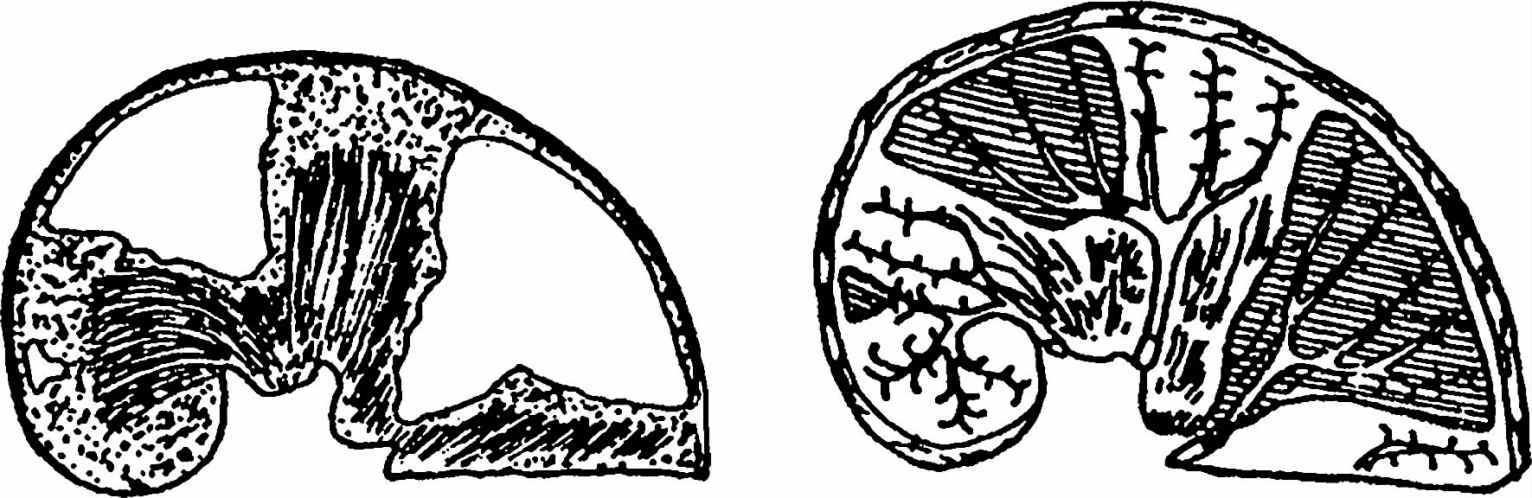
\includegraphics{./images/Image00046.jpg}
  \caption{肾动脉分支阻塞及贫血性梗死示意图}
  \label{fig3-12}
\end{figure}


\subsubsection{梗死的类型}

根据梗死区内含血量的多少,可将梗死分为贫血性梗死及出血性梗死。

\paragraph{贫血性梗死(anemic infarct)}
多发生于侧支循环不充分,且组织结构较致密的实质性器官,如心、肾、脾,有时也可发生于脑。当梗死形成时,该供血区内及邻近的动脉分支发生反射性痉挛,使该区内原有的血液被排挤到周围组织中呈贫血状态。缺血区的组织坏死呈灰白或灰黄色,故贫血性梗死亦称为白色梗死。

发生于脾、肾的梗死灶多呈锥形,切面呈楔形,尖端指向血管阻塞的部位,底部位于脏器的表面,浆膜面常有纤维素性渗出物覆盖。发生于心肌的梗死灶呈不规则地图状。梗死的早期,在梗死灶边缘因炎症反应常可见一充血出血带围绕,数日后因血红蛋白分解转变为含铁血黄素而变成一棕黄色带。陈旧性梗死灶由于机化和瘢痕收缩,病灶表面下陷,质地变坚实,充血出血带消失。镜下,梗死组织呈凝固性坏死,早期仍可见到组织结构的模糊轮廓,但细胞结构消失。梗死灶周围与正常组织交界处除可见充血、出血带外,还有较多中性粒细胞浸润(图\ref{fig3-13})。晚期,充血出血带消失,梗死灶内有肉芽组织长入,最后形成瘢痕。

\begin{figure}[!htbp]
  \centering
  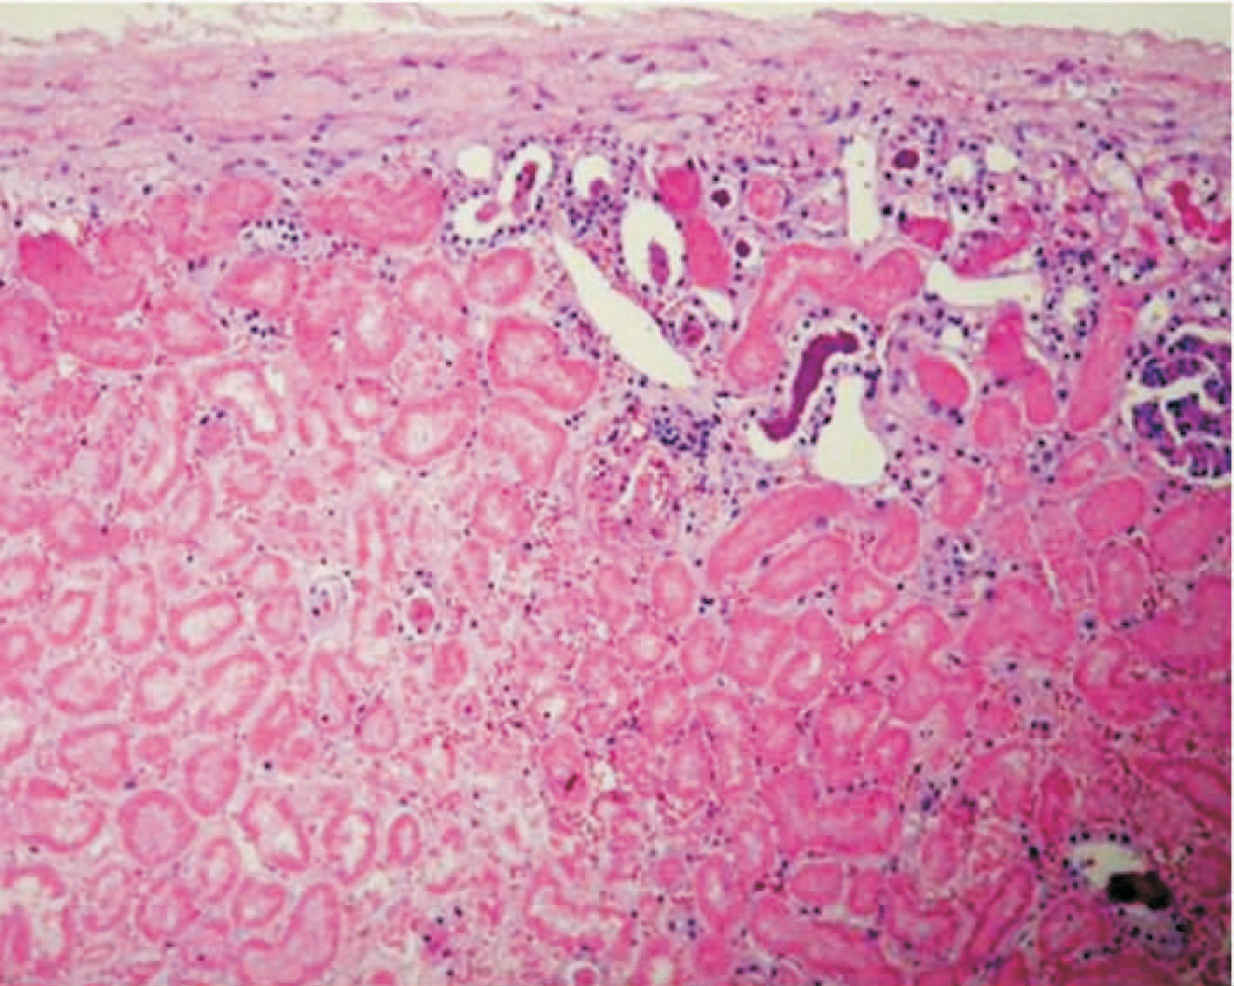
\includegraphics{./images/Image00047.jpg}
  \caption{肾贫血性梗死(HE染色,低倍) \\ {\small 左下方梗死灶呈凝固性坏死}}
  \label{fig3-13}
\end{figure}

脑梗死一般为贫血性梗死,坏死的脑组织因含脂质及水分较多,不易凝固,常软化、液化而后形成囊腔,或被胶质细胞及其纤维所代替,最后形成胶质瘢痕。

\paragraph{出血性梗死(hemorrhagic infarct)}
多发生于肺、肠等具有双重血液循环、组织结构疏松的器官,且伴有严重淤血的情况下,因在梗死灶内常有明显的出血,故称为出血性梗死,亦称红色梗死。

出血性梗死的形成,除动脉血流阻断这一基本原因外,还与严重的静脉淤血、具有双重血液循环或侧支循环丰富及组织结构疏松等条件有关。如肺和肠,在正常情况下,即使其中一支动脉被阻塞,另一支动脉尚可维持血液供应,不致发生梗死。但当脏器发生严重淤血时,由于整个器官的静脉和毛细血管内压增高,阻碍了吻合支中动脉血液的流入,因此,不能建立有效的侧支循环,引起局部组织器官的缺血、缺氧而发生梗死。同时,由于严重的淤血及组织结构疏松,梗死发生后,梗死区的血管破坏,可导致弥漫性出血。

(1)肺出血性梗死:多发生于已有严重肺淤血(如风湿性心脏病二尖瓣病变)的基础上再有肺动脉栓塞。栓子多来自下肢静脉、右心或子宫静脉的血栓。多发生于肺下叶外周部,尤以肋膈角处多见。肉眼观,梗死部隆起,呈暗紫红色,质较实,呈锥体形。切面为楔形,尖端指向肺门或血管阻塞处,基底位于胸膜面。胸膜表面常有纤维素渗出。镜下,梗死区肺泡间隔结构模糊不清,肺泡腔内和组织间隙充满红细胞,周围肺组织多有慢性淤血及水肿(图\ref{fig3-14})。

\begin{figure}[!htbp]
  \centering
  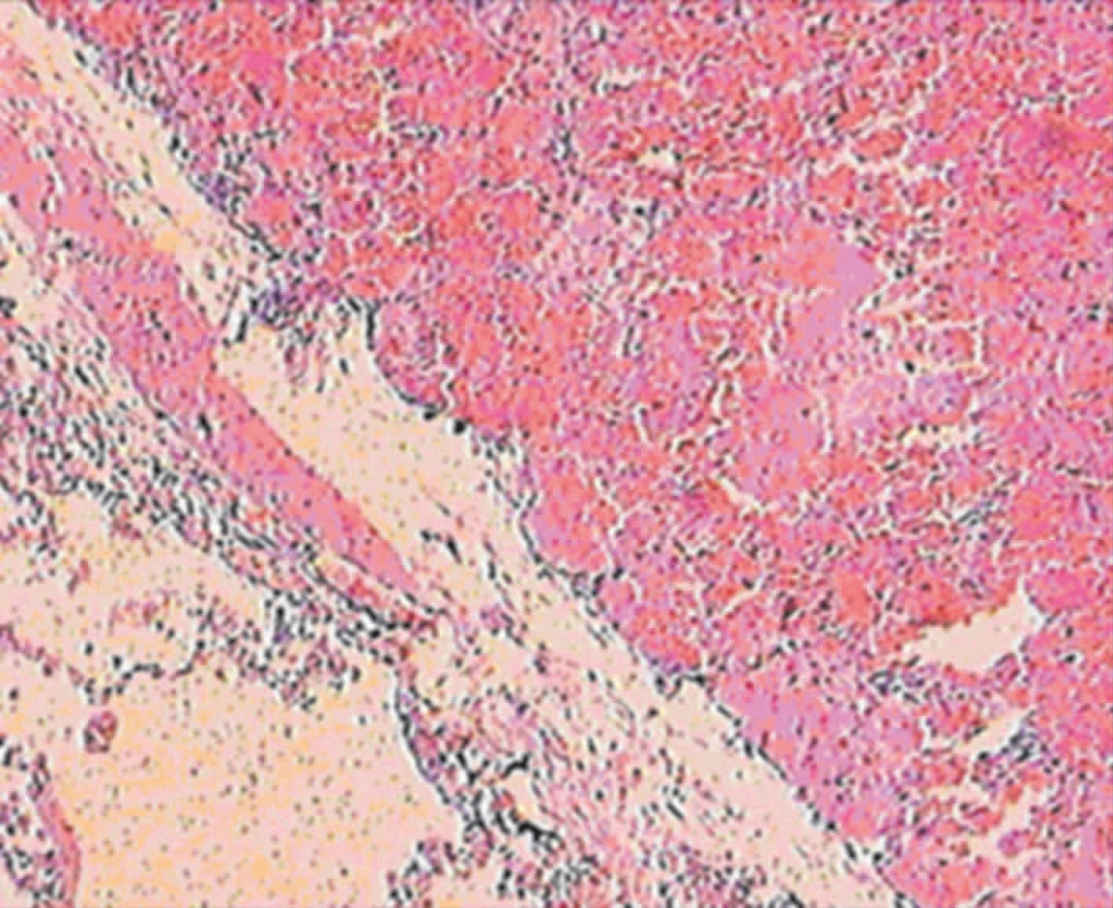
\includegraphics{./images/Image00048.jpg}
  \caption{肺出血性梗死(HE染色,低倍) \\ {\small 右上方梗死区肺组织出血、坏死}}
  \label{fig3-14}
\end{figure}


肺梗死的结局因梗死区的大小及数目多少而异。较小的梗死,病人可出现胸痛及咯血等症状;较大区域的梗死可引起呼吸困难。因肺组织借支气管与外界相通,故在梗死的基础上易继发感染。

(2)肠出血性梗死:多发生于肠扭转、肠套叠、绞窄性肠疝等情况下。这时,因静脉首先受压而发生高度淤血,继而,动脉亦受压阻断而造成出血性梗死。肠梗死多发生于小肠,通常只累及小肠的某一肠段,长短不等,梗死的肠壁因弥漫性出血而呈紫红或红黑色。因有显著淤血、水肿及出血,使肠壁肿胀增厚,质脆弱,易破裂。肠腔内充满混浊的暗红色液体,在浆膜面可有纤维素性渗出物。

梗死早期,由于组织缺血,肠壁肌肉发生痉挛性收缩,可致剧烈腹痛。梗死后,肠蠕动消失,可引起腹胀、呕吐等肠梗阻症状。此时如不及时处理,肠道内的内容物及细菌等可经坏死的肠壁进入腹腔,引起弥漫性腹膜炎,造成严重后果。

贫血性梗死和出血性梗死的区别见表\ref{tab3-2}。
\begin{table}[ht]
  \caption{贫血性梗死和出血性梗死的区别}
  \label{tab3-2}
  \centering
  \begin{tabular}{lp{5cm}p{5cm}}
    \toprule
    区别要点 & 贫血性梗死
             & 出血性梗死                                                                                     \\
    \midrule
    病因     & 动脉阻塞                                          &
    高度淤血基础上的动脉阻塞                                                                                  \\
    好发器官 & 肾、脾、心脏等
             & 肺、肠等                                                                                       \\
    血供情况 & 血管吻合支少                                      & 双重血供或血管吻合支丰富                   \\
    肉眼形态 & 灰白色,梗死灶内无出血                            & 暗红色,梗死灶内明显出血                   \\
    组织结构 & 实质性,比较致密,组织轮廓可见;周围充血.出血带明显 & 比较疏松,组织轮廓不清;周围充血出血带不明显 \\
    \bottomrule
  \end{tabular}
\end{table}

此外,尚可根据梗死灶内有无合并细菌感染而将梗死分为单纯性梗死和败血性梗死。若在梗死灶内有大量细菌生长繁殖,引起急性炎症反应,称为败血性梗死。主要由含有细菌的栓子阻塞血管所致,常见于急性感染性心内膜炎时,心脏瓣膜上含有细菌的赘生物脱落引起栓塞所致的梗死。如为化脓菌感染,则可有脓肿形成。

\subsection{梗死对机体的影响和结局}

梗死对机体的影响,取决于发生梗死的器官、梗死的大小和部位。肾、脾的梗死一般影响小。肾梗死通常出现腰痛和血尿,不影响肾功能;肺梗死有胸痛和咯血;肠梗死常出现剧烈腹痛、血便和腹膜炎的症状;心肌梗死影响心脏功能,严重者可导致心力衰竭甚至猝死;脑梗死出现相应部位功能障碍,梗死灶大者可致死。

梗死是局部组织由于血流阻断而发生的坏死,因此,梗死的结局如同坏死的结局,即梗死灶周围发生急性炎症反应,小的梗死灶可被肉芽组织完全取代而机化,日久形成瘢痕。大的梗死灶不能完全机化时,则由肉芽组织和瘢痕组织加以包裹,病灶内可发生钙化。

\section*{复习与思考}

{一、名词解释}

淤血 心衰细胞 槟榔肝 肺褐色硬化 血栓形成 附壁血栓 再通 栓塞 减压病 梗死

{二、问答题}

1. 淤血有哪些主要后果?

2. 试述血栓形成的条件。

3. 试述各种类型血栓的形态特点。

4. 栓子有哪些类型?其中哪一种最常见?说明栓子的运行途径。

5. 试述梗死主要类型的形态特点。

6. 试述血栓形成、栓塞及梗死之间的联系。

{三、临床病理讨论}

病史摘要:女性患者,52岁,农民,患风湿性心脏病二尖瓣狭窄10余年。近年来心功能一直不好。半年前出现右侧肢体偏瘫。近日呼吸困难加重,咳嗽,咳粉红色泡沫样痰,咯血,肝脾肿大,全身水肿,胸腹腔积液。经住院治疗无效死亡。

尸检所见:(主要脏器改变)

肉眼观:右肺下叶可见暗红色实性病灶,切面呈楔形,病灶底部靠近胸膜,尖端朝向肺门,边界清楚。左肺动脉大分支有两支血管内见暗红色固形物阻塞。心脏体积明显增大,重量增加,左心房、右心室和右心房明显扩张,左心房后壁局部粗糙,有凝血块样物附着。二尖瓣瓣膜增厚、变硬、变形,瓣口狭窄。左侧大脑内囊部脑组织灶性软化。

镜下:肺组织实性病灶内有明显的出血坏死,坏死灶内肺组织轮廓尚依稀可见。病灶周围肺组织高度淤血。左肺动脉分支内固形物为红色血栓成分。左心房后壁凝血块样物为附壁血栓。内囊部灶性软化的脑组织为液化性坏死。

讨论题:

1. 本例的病理诊断是什么?

2. 试分析其主要疾病的发生发展过程。

3. 右侧肢体偏瘫和肺出血坏死分别是如何形成的?

4. 试分析本例的死亡原因和可能机制。

